\documentclass[conference]{IEEEtran}
\usepackage{amsmath}
\usepackage{graphicx}
\usepackage{booktabs}
\usepackage{siunitx}
\usepackage[hidelinks]{hyperref}
\graphicspath{{figures/}}
\sisetup{group-minimum-digits=4}

% house style: no em dashes, so the abstract heading uses a colon
\makeatletter
\def\abstract{\normalfont\@IEEEabskeysecsize\bfseries\textit{\abstractname}:\ \relax\@IEEEgobbleleadPARNLSP}
\makeatother

\newcommand{\ugm}{\si{\micro\gram\per\cubic\metre}}

% allow more floats per page so tables and figures stay near their text
\renewcommand{\topfraction}{0.85}
\renewcommand{\bottomfraction}{0.6}
\renewcommand{\textfraction}{0.1}
\renewcommand{\floatpagefraction}{0.75}
\setcounter{topnumber}{3}
\setcounter{bottomnumber}{2}
\setcounter{totalnumber}{5}

\begin{document}

\title{Data understanding and leak-free preprocessing for short-horizon PM2.5 forecasting in Beijing}

\author{\IEEEauthorblockN{Vetriselvan R, Hrishi Dongre, Pampana Sree Adithya, Ishan Goyal, Vedant Madne}
\IEEEauthorblockA{Team T024, Section A - AML/DL Project 19: Air quality forecasting via gradient boosting and LSTM models}}

\maketitle

\begin{abstract}
We analyse and prepare the UCI Beijing PM2.5 hourly dataset (2010 to 2014) for a forecasting study that compares gradient boosting with recurrent models. Exploratory analysis runs on the original file in two scopes: data-quality checks on all five years, and pattern analysis on 2010 to 2013 only, so that the 2014 test year never shapes a decision. The data quality checks find a complete hourly grid, missing values only in the target (4.72\%, 214 gaps, most of them short), a measurable cost of filling gaps (13~\ugm{} after one hour, 27 after three), and three weather columns stored as running totals. The pattern analysis finds opposite daily cycles in winter and summer, strong but fading persistence (lag-1 autocorrelation 0.96, lag-24 0.33), humidity and wind as the main weather drivers, 322 pollution episodes that build slowly and clear quickly under north-west wind, and Lunar New Year spikes of 7 to 14 times the usual level. Every finding is mapped to a preprocessing or modelling decision. The pipeline decodes the running totals, keeps the label untouched beside a causal input copy filled for at most three hours, builds expanding-window folds with a 24-hour embargo, and fits scaling on training rows only. Automated tests and an independent two-reviewer leakage audit verify these guarantees.
\end{abstract}

\section{Introduction}
The project forecasts hourly PM2.5 concentration a few hours ahead from past pollution and weather, and compares an XGBoost model (Phase 1) with an LSTM or temporal CNN (Phase 2) under chronological backtesting. Such comparisons are only meaningful if no information from the evaluation period reaches training, whether through filling, scaling, the split or the analyst's own choices \cite{kaufman2012,tashman2000,bergmeir2012}. This report covers the data stage and follows the order of the work, which is also the order of the project notebooks: exploratory data analysis (EDA) first \cite{tukey1977}, then preprocessing driven by its findings, then modelling.

Our contributions are:
\begin{itemize}
\item an EDA of the original file with an explicit scope rule that keeps the test year out of every decision (Sections~\ref{sec:protocol} to \ref{sec:patterns});
\item a traceable mapping from each finding to a preprocessing or modelling decision (Tables~\ref{tab:prep} and \ref{tab:model});
\item a leak-free preprocessing pipeline (Section~\ref{sec:prep});
\item verification by automated tests and an independent leakage review (Section~\ref{sec:verify}).
\end{itemize}

\section{Dataset}
The dataset \cite{uci} holds hourly PM2.5 measured at the US Embassy in Beijing together with meteorology from Beijing Capital International Airport, from 2010-01-01 00:00 to 2014-12-31 23:00 (\num{43824} rows). It was introduced in \cite{liang2015}. Table~\ref{tab:cols} lists the variables; column names are shortened when loading and values are not changed. The years 2010 to 2013 are the development years, used for training and for three validation folds; 2014 is the test year, held out and scored once at the end.

\begin{table}[!htb]
\centering
\caption{Variables}
\label{tab:cols}
\begin{tabular}{@{}lll@{}}
\toprule
Name & Raw & Meaning (unit) \\
\midrule
pm25 & pm2.5 & PM2.5 concentration (\ugm), target \\
dewp & DEWP & dew point (\si{\celsius}) \\
temp & TEMP & temperature (\si{\celsius}) \\
pres & PRES & pressure (hPa) \\
cbwd & cbwd & combined wind direction: NE, NW, SE, cv \\
ws\_cum & Iws & cumulated wind speed (m/s) \\
snow\_cum & Is & cumulated hours of snow \\
rain\_cum & Ir & cumulated hours of rain \\
\bottomrule
\end{tabular}
\end{table}

\section{Analysis protocol}
\label{sec:protocol}
The EDA reads the original csv and writes nothing. It has two scopes.
\begin{itemize}
\item \textbf{Data quality, all years.} How the data was recorded: the time grid, missing values and gaps, value ranges, and what the unusual columns contain. These facts describe the file, not the behaviour of PM2.5, so the whole file is checked.
\item \textbf{Patterns, 2010 to 2013 only.} Anything that describes how PM2.5 behaves or that shapes a modelling choice, including the cost of filling gaps, skew, typical wind speeds, cycles and drivers. Looking at test-year patterns before the final score is a quiet form of leakage \cite{kaufman2012}, so 2014 is excluded.
\end{itemize}
A few helper columns are computed inside the EDA for analysis only: hourly wind speed (Section~\ref{sec:cum}), relative humidity from temperature and dew point with the Magnus formula \cite{alduchov1996}, and snow and rain flags. They are not saved; the pipeline builds its own versions.

\section{Data quality}
\label{sec:quality}

\subsection{Grid and missing values}
The file has one row per hour, with no duplicates and no skipped hours, so the grid only has to be verified, not resampled. Only pm25 has missing values: \num{2067} hours (4.72\%). Every weather column is complete. Missingness falls from 669, 728 and 489 hours in 2010, 2011 and 2012 to 82 and 99 in 2013 and 2014 (Fig.~\ref{fig:missing}). Table~\ref{tab:gaps} groups the 214 gaps by length: most are short, while 20 gaps longer than a day hold 65\% of the missing hours. The longest gap lasts 155 hours from 2010-09-21 05:00.

\begin{figure}[!t]
\centering
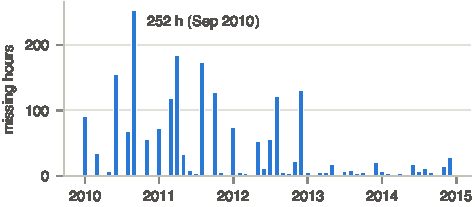
\includegraphics[width=\columnwidth]{missing.pdf}
\caption{Missing pm25 hours per month, all years. Gaps concentrate in 2010 to 2012.}
\label{fig:missing}
\end{figure}

\begin{table}[!htb]
\centering
\caption{Gaps in pm25 by length, all years}
\label{tab:gaps}
\begin{tabular}{@{}lrrrrr@{}}
\toprule
Length & 1 h & 2--3 h & 4--6 h & 7--24 h & $>$24 h \\
\midrule
Gaps & 112 & 31 & 15 & 36 & 20 \\
Missing hours & 112 & 64 & 74 & 476 & \num{1341} \\
\bottomrule
\end{tabular}
\end{table}

\subsection{Cost of filling a gap}
Carrying the last observed value forward $k$ hours is exactly a persistence guess $k$ hours ahead, so its mean absolute error on observed hours measures how wrong a filled value would be (Table~\ref{tab:fill}, 2010 to 2013). Up to three hours the fill stays close to the truth; beyond that it starts to invent data. Linear interpolation is not an option, because it uses the first value after the gap, which a forecaster would not yet have.

\begin{table}[!htb]
\centering
\caption{Mean absolute error of carrying a value forward (\ugm), 2010 to 2013}
\label{tab:fill}
\begin{tabular}{@{}lrrrrrr@{}}
\toprule
Hours carried & 1 & 2 & 3 & 4 & 6 & 12 \\
\midrule
Error & 13.1 & 20.9 & 27.0 & 32.3 & 40.8 & 56.3 \\
\bottomrule
\end{tabular}
\end{table}

\subsection{Ranges and extremes}
All ranges are physically plausible: dew point $-40$ to 28~\si{\celsius}, temperature $-19$ to 42~\si{\celsius}, pressure 991 to 1046~hPa, pm25 0 to 994. The two highest pm25 values, 994 at 2012-01-23 01:00 and 980 at 2010-02-14 01:00, fall in the first hours of Lunar New Year, and their neighbours rise and fall with them (225, 994, 972, 430 from midnight to 03:00 in 2012), so they are fireworks pollution, not sensor errors. Only two hours are exactly 0. Nothing is clipped or removed.

\subsection{Cumulative columns}
\label{sec:cum}
Iws is described as cumulated wind speed. It falls in \num{8283} hours, every one of them at a change of wind direction, and it rises in every hour inside a direction run. It is therefore a running total per direction run, not a wind speed (Fig.~\ref{fig:wind}). With $d_t$ the direction and $I_t$ the Iws value at hour $t$, the hourly speed is
\begin{equation}
ws_t = \begin{cases} I_t & d_t \neq d_{t-1} \\ I_t - I_{t-1} & d_t = d_{t-1} \end{cases}
\label{eq:ws}
\end{equation}
Is and Ir are counters of snow and rain hours. They are 0 in 99.2\% and 95.9\% of hours, and in 6 of 368 and 53 of \num{1808} positive hours they jump instead of rising by one. A value above zero reliably means snow or rain is falling in that hour.

\begin{figure}[!t]
\centering
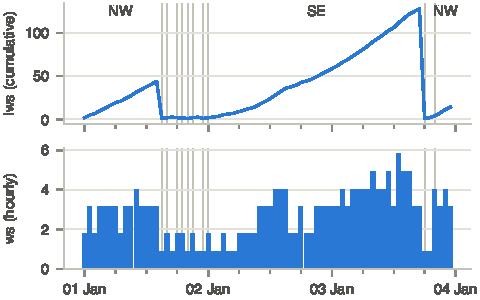
\includegraphics[width=\columnwidth]{wind_decode.pdf}
\caption{First three days of 2010. Top: raw Iws, a running total that restarts at each direction change (vertical lines; long runs labelled). Bottom: hourly speed recovered with (\ref{eq:ws}), in m/s.}
\label{fig:wind}
\end{figure}

\subsection{Wind directions and skew}
cbwd has four levels, NE (\num{4997} hours), NW (\num{14150}), SE (\num{15290}) and cv (\num{9387}), with no south-west level. cv hours average 0.99~m/s in 2010 to 2013, consistent with ``calm and variable''. pm25 and the wind columns are strongly right-skewed (Table~\ref{tab:skew}, Fig.~\ref{fig:hist}): a few very high values would dominate a squared-error loss, and log1p, $\log(1+x)$, removes most of the skew. The snow and rain counters stay skewed because they are almost always zero; the flags are their useful form.

\begin{table}[!htb]
\centering
\caption{Skewness before and after log1p, 2010 to 2013}
\label{tab:skew}
\begin{tabular}{@{}lrrrrr@{}}
\toprule
 & pm25 & ws & ws\_cum & snow\_cum & rain\_cum \\
\midrule
Raw & 1.81 & 1.72 & 4.19 & 18.45 & 11.39 \\
log1p & $-0.29$ & 0.48 & 0.67 & 12.19 & 6.01 \\
\bottomrule
\end{tabular}
\end{table}

\begin{figure}[!t]
\centering
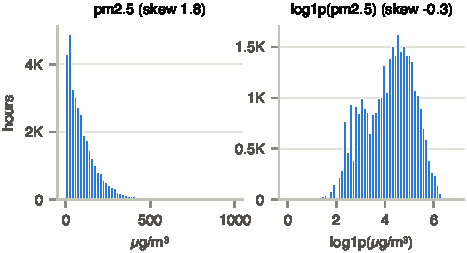
\includegraphics[width=\columnwidth]{target_hist.pdf}
\caption{Distribution of pm25 before and after log1p, 2010 to 2013.}
\label{fig:hist}
\end{figure}

\section{Patterns, 2010 to 2013}
\label{sec:patterns}

\subsection{Level and trend}
There is no trend across the development years: the yearly mean is 104.0, 99.1, 90.5 and 101.7~\ugm{} for 2010 to 2013. The variation sits inside each year, with daily means moving from clean days to several hundred within a week (Fig.~\ref{fig:daily}). Using the PM2.5 breakpoints of China's air quality standard HJ 633-2012 \cite{hj633} on single hours (the standard uses 24-hour means, so this is for context only; on 2026-03-01 it was replaced by HJ 633-2026, which revises the PM2.5 limits), 51.4\% of hours are excellent or good ($\le 75$) and 21.9\% are heavily or severely polluted ($>150$).

\begin{figure}[!t]
\centering
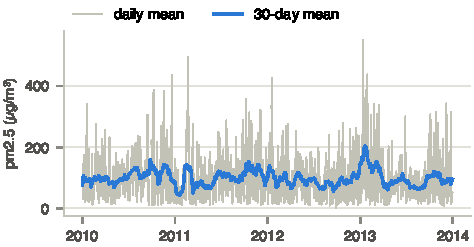
\includegraphics[width=\columnwidth]{daily.pdf}
\caption{Daily mean pm25 and its 30-day mean, 2010 to 2013.}
\label{fig:daily}
\end{figure}

\subsection{Cycles}
Winter and summer have opposite daily shapes (Fig.~\ref{fig:diurnal}). In winter the median peaks at 21:00 (96~\ugm) and is lowest from 12:00 to 15:00 (47); in summer it peaks at 08:00 (94) and is lowest at 17:00 (70). Hour of day therefore matters only together with the season. In January and December the mean is almost twice the median (114.1 against 59, 103.2 against 60; Fig.~\ref{fig:monthly}): winter mixes very clean days with severe episodes. Day of week matters little, with means from 93.5 (Thursday) to 103.2 (Saturday).

\begin{figure}[!t]
\centering
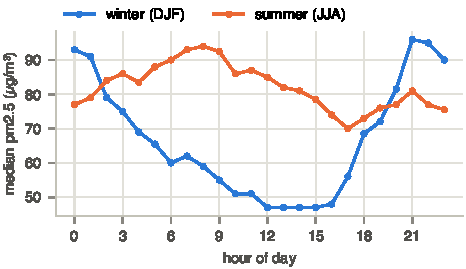
\includegraphics[width=\columnwidth]{diurnal.pdf}
\caption{Median pm25 by hour of day, winter (DJF) and summer (JJA).}
\label{fig:diurnal}
\end{figure}

\begin{figure}[!t]
\centering
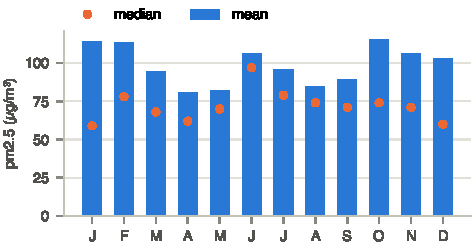
\includegraphics[width=\columnwidth]{monthly.pdf}
\caption{Mean and median pm25 by month.}
\label{fig:monthly}
\end{figure}

\subsection{Persistence}
The autocorrelation of log1p(pm25) is 0.96 at one hour, 0.74 at six and 0.33 at 24 (Fig.~\ref{fig:acf}). The partial autocorrelation, which removes what shorter lags already explain, is dominated by lag 1, with a small correction at lag 2 ($-0.10$) and a faint daily echo at lags 24 and 25 ($-0.02$, $-0.03$); for this one calculation remaining gaps are carried forward. Copying the current value is wrong by 13.1, 40.8 and 69.8~\ugm{} at 1, 6 and 24 hours ahead (Table~\ref{tab:persist}). A seasonal-naive guess (the same hour one day earlier) is wrong by about 70 at every horizon, so it only ties with persistence at 24 hours.

\begin{figure}[!t]
\centering
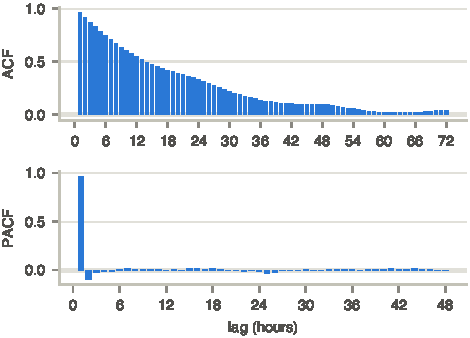
\includegraphics[width=\columnwidth]{acf_pacf.pdf}
\caption{Autocorrelation and partial autocorrelation of log1p(pm25). The grey band is the 95\% range for white noise.}
\label{fig:acf}
\end{figure}

\begin{table}[!htb]
\centering
\caption{Error of naive forecasts by horizon (\ugm), 2010 to 2013}
\label{tab:persist}
\begin{tabular}{@{}lrrrrrr@{}}
\toprule
Horizon (h) & 1 & 2 & 3 & 6 & 12 & 24 \\
\midrule
Persistence MAE & 13.1 & 20.8 & 27.0 & 40.8 & 56.4 & 69.8 \\
Seasonal-naive MAE & 69.8 & 69.9 & 69.9 & 69.9 & 69.8 & 69.8 \\
Lag-$h$ correlation (raw) & 0.96 & 0.92 & 0.87 & 0.74 & 0.55 & 0.39 \\
\bottomrule
\end{tabular}
\end{table}

\subsection{Weather}
Calm (cv) and south-east winds bring the dirtiest air (median 100 and 93~\ugm), north-west the cleanest (31), and pm25 falls steadily as wind speed rises to about 6~m/s (Fig.~\ref{fig:windfx}). Relative humidity is the strongest single weather signal (Table~\ref{tab:spear}); median pm25 climbs from 21 in air below 20\% humidity to 129 above 90\%. Temperature, rain and snow alone show almost no rank correlation.

\begin{figure}[!t]
\centering
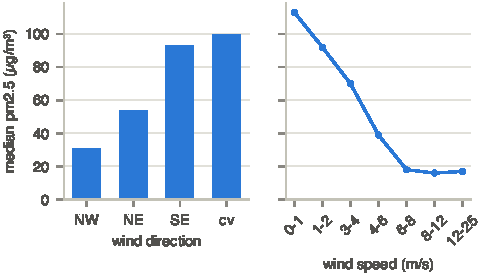
\includegraphics[width=\columnwidth]{wind_effect.pdf}
\caption{Median pm25 by wind direction (left) and by hourly wind speed (right).}
\label{fig:windfx}
\end{figure}

\begin{table}[!htb]
\centering
\caption{Spearman correlation with pm25 now and six hours later}
\label{tab:spear}
\begin{tabular}{@{}lrrrrrr@{}}
\toprule
 & rh & ws & ws\_cum & dewp & pres & temp \\
\midrule
pm25 at $t$ & 0.54 & $-0.46$ & $-0.38$ & 0.33 & $-0.17$ & 0.04 \\
pm25 at $t+6$ & 0.39 & $-0.46$ & $-0.34$ & 0.27 & $-0.14$ & 0.07 \\
\bottomrule
\end{tabular}
\end{table}

\subsection{What predicts the next six hours}
Table~\ref{tab:next6} groups the change from $t$ to $t+6$ by conditions known at $t$. South-east wind tends to raise pm25 and north-west wind to lower it. The first three hours of a north-west spell are the strongest clearing signal, while spells older than a day see pm25 rising again, so how long the wind has blown matters as well as its direction. Pressure rising by more than 2~hPa in three hours, typical of a cold front, gives the largest drop.

\begin{table}[!htb]
\centering
\caption{Change of pm25 over the next six hours, 2010 to 2013}
\label{tab:next6}
\begin{tabular}{@{}llrr@{}}
\toprule
Condition at $t$ & Group & Median change & Halving \\
\midrule
Wind direction & SE & $+16.8\%$ & 7.3\% \\
 & cv & $+7.2\%$ & 11.8\% \\
 & NE & $+3.1\%$ & 14.1\% \\
 & NW & $-4.3\%$ & 18.5\% \\
\midrule
Age of NW spell & 1--3 h & $-12.2\%$ & 24.0\% \\
 & 4--6 h & $-9.5\%$ & 22.2\% \\
 & 7--12 h & $+0.6\%$ & 14.4\% \\
 & 13--24 h & $+10.0\%$ & 10.0\% \\
 & $>$24 h & $+17.6\%$ & 4.2\% \\
\midrule
Pressure change & $\le -1$ hPa & $+17.8\%$ & 8.3\% \\
over 3 h & $-1$ to 0 & $+4.7\%$ & 11.9\% \\
 & 0 to 1 & $+0.1\%$ & 15.4\% \\
 & 1 to 2 & $-1.2\%$ & 19.5\% \\
 & $>2$ hPa & $-21.4\%$ & 25.8\% \\
\bottomrule
\multicolumn{4}{@{}p{0.95\columnwidth}@{}}{\footnotesize Halving: share of hours where pm25 at $t+6$ is below half of pm25 at $t$.}
\end{tabular}
\end{table}

\subsection{Pollution episodes}
We call an episode a run of at least six consecutive hours above 150~\ugm{} (a working definition, not an official one). There are 322 episodes covering 19\% of observed hours, with median duration 14 hours and a longest of 111. They build slowly, a median 55 hours from the lowest value of the previous 72 hours to the peak (a lower bound set by the 72-hour window), and clear fast, a median 14 hours to fall below a quarter of the peak. North-west wind blows at 54.9\% of clearings against 33.4\% of all hours, while south-east wind is under-represented (19.1\% against 34.4\%). Fig.~\ref{fig:episode} shows this saw-tooth pattern. Episode hours are where large forecast errors will come from, so models are also scored on them separately.

\begin{figure}[!t]
\centering
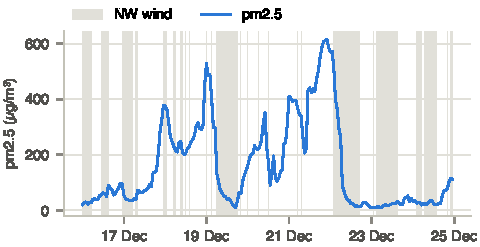
\includegraphics[width=\columnwidth]{episode.pdf}
\caption{Two episodes in December 2010: slow build-up, then collapse when north-west wind (shaded) arrives.}
\label{fig:episode}
\end{figure}

\subsection{Lunar New Year}
Every year the peak on the eve or first day of Lunar New Year is 7 to 14 times the median of the surrounding two weeks (Table~\ref{tab:lny}), always between 22:00 and 01:00. No weather variable explains these spikes, so only a calendar flag lets a model expect them.

\begin{table}[!htb]
\centering
\caption{Lunar New Year peaks (\ugm)}
\label{tab:lny}
\begin{tabular}{@{}lrlr@{}}
\toprule
New Year's day & Peak & Peak hour & Median, $\pm$8 days \\
\midrule
2010-02-14 & 980 & 14 Feb 01:00 & 68.0 \\
2011-02-03 & 348 & 3 Feb 01:00 & 42.0 \\
2012-01-23 & 994 & 23 Jan 01:00 & 76.0 \\
2013-02-10 & 512 & 9 Feb 22:00 & 70.5 \\
\bottomrule
\end{tabular}
\end{table}

\subsection{Redundancy and stationarity}
Dew point, temperature and pressure move together (Pearson $|r|$ from 0.78 to 0.83), which does not hurt tree models but makes linear coefficients unstable, so linear models need regularisation. An augmented Dickey-Fuller test \cite{dickey1979} on daily mean log1p(pm25) gives a statistic of $-22.2$ ($p<0.001$, \num{1424} daily means): the series is stationary around a stable level, so models can work on log1p levels with lags and no differencing.

\section{Preprocessing}
\label{sec:prep}
Table~\ref{tab:prep} lists the decisions taken from Section~\ref{sec:quality}. The pipeline is a Python package (src/aqf/data) driven by one configuration file and run with \texttt{python -m aqf.data.pipeline}; notebook 02 walks through it step by step.

\begin{table}[!htb]
\centering
\caption{Data-quality findings and preprocessing decisions}
\label{tab:prep}
\begin{tabular}{@{}p{0.43\columnwidth}p{0.49\columnwidth}@{}}
\toprule
Finding & Decision \\
\midrule
Complete hourly grid & Validate it and fail loudly; no resampling \\
Only pm25 missing & Validate that weather stays complete \\
Iws is a running total & Decode hourly ws with (\ref{eq:ws}); keep ws\_cum \\
Is, Ir are counters & Snow and rain flags (counter $>0$); keep counters \\
Four wind levels & One-hot in fixed order NE, NW, SE, cv \\
Missing labels are unknowable & Never fill the label; skip those hours \\
Filling costs 13 at 1 h, 27 at 3 h & Causal input copy, carried forward at most 3 h \\
Interpolation uses the future & No interpolation \\
Missingness uneven over time & Missing flag as a model input \\
Extremes are real & Keep them; no clipping \\
pm25 and wind columns skewed & log1p before scaling \\
\bottomrule
\end{tabular}
\end{table}

\subsection{Validation, decoding and encoding}
The loader checks the exact column list, builds the timestamp index from year, month, day and hour, and stops with an error if the hourly grid has holes or duplicates or if any weather value is missing, so the pipeline fails rather than silently repairing data. Iws is decoded with (\ref{eq:ws}); decoded speeds lie between 0.45 and 20.12~m/s. The running total stays as ws\_cum because it also encodes how long the wind has blown from one direction. Snow and rain become flags next to their counters, and cbwd is one-hot encoded in a fixed order, so column positions never depend on which levels appear in a fold.

\subsection{Missing target values}
The label pm25 is never filled; a missing label means the hour is excluded from training loss and evaluation. A flag pm25\_miss records the original missingness, and an input column pm25\_in carries the last observed value forward for at most $L=3$ hours:
\begin{equation}
\tilde{y}_t = y_{t-k}, \quad k = \min\{j \ge 0 : y_{t-j}\ \text{observed}\}, \quad k \le L,
\end{equation}
staying missing otherwise. This recovers 386 input hours; \num{1681} stay missing for the model stage (XGBoost handles missing inputs natively).

\subsection{Chronological folds with an embargo}
Following rolling-origin evaluation \cite{tashman2000,hyndman2021}, fold $k$ evaluates on calendar year $Y_k$ and trains on all hours in $[t_0,\ s_k - G)$, where $s_k$ is 1 January of $Y_k$ and $G = 24$ hours is a gap that we call the embargo. With $G$ at least the forecast horizon, every training row whose target would fall inside the evaluation year is dropped, which L\'{o}pez de Prado calls purging \cite{lopezdeprado2018}. Whole years give every fold a full seasonal cycle, and 2014 is the test year (Fig.~\ref{fig:folds}, Table~\ref{tab:folds}).

\begin{figure}[!t]
\centering
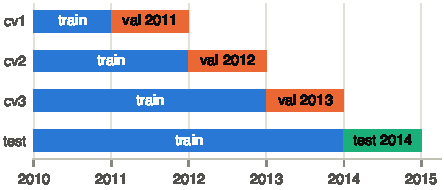
\includegraphics[width=\columnwidth]{folds.pdf}
\caption{Expanding-window folds. The 24-hour embargo before each evaluation year is too short to see at this scale.}
\label{fig:folds}
\end{figure}

\begin{table}[!htb]
\centering
\caption{Folds (hours)}
\label{tab:folds}
\begin{tabular}{@{}lllrr@{}}
\toprule
Fold & Last training hour & Evaluate & Train & Labelled eval \\
\midrule
cv1 & 2010-12-30 23:00 & 2011 & \num{8736} & \num{8032} \\
cv2 & 2011-12-30 23:00 & 2012 & \num{17496} & \num{8295} \\
cv3 & 2012-12-30 23:00 & 2013 & \num{26280} & \num{8678} \\
test & 2013-12-30 23:00 & 2014 & \num{35040} & \num{8661} \\
\bottomrule
\end{tabular}
\end{table}

\subsection{Leak-free scaling and outputs}
For each fold a scaler is fitted on that fold's training rows only:
\begin{equation}
z = \frac{g(x) - \mu_{\text{train}}}{\max(\sigma_{\text{train}}, \epsilon)},
\end{equation}
where $g$ is log1p for the skewed columns (pm25, pm25\_in, ws, ws\_cum, snow\_cum, rain\_cum) and the identity otherwise. Tree models do not need it; recurrent models do, and predictions are mapped back to \ugm{} before computing MAE, RMSE and $R^2$. The pipeline writes the cleaned hourly table (data/interim/hourly.parquet), the fold boundaries and one scaler per fold (data/processed), and the audit numbers (reports/data/qa.json). Statistics that must be learned per fold, such as scalers or an hour-of-day climatology, cannot be computed once for the whole file without leaking, so the fold-dependent features are built at the modelling stage inside each fold.

\section{Verification}
\label{sec:verify}

\subsection{Automated tests}
Nine tests check that: the grid is complete and hourly; only the target is missing; summing decoded speeds within each direction run rebuilds Iws exactly; the one-hot columns are exclusive; the label is unchanged and the flag matches it; filling at hour $t$ is identical whether or not later hours exist; folds never overlap and respect the embargo; the pipeline's scalers do not change when every row from the end of a fold's training span onward is altered; and a scaler round-trips through disk and its inverse.

\subsection{Independent leakage review}
Two reviewers audited the work separately, one for the data stage and one for the modelling stage, using code reading and perturbation checks. The data-stage review confirmed that every cleaning step looks only backward (cleaning the file cut at several points reproduces the full result exactly), that the saved scalers equal fits on training rows only, and that no training span contains 2014. It found three issues, all fixed: the skew that justifies log1p had been measured on all five years (now 2010 to 2013; the decision is unchanged, 1.81 against 1.80); one fill-cost calculation shifted values before excluding 2014; and the scaler test passed by construction (it now perturbs later rows through the pipeline's own function). The modelling-stage review found that validation rows at the end of 2013 were scored against labels from the first hours of 2014; this is fixed and reported with the models.

\section{Implications for modelling}
Table~\ref{tab:model} maps the pattern findings to the Phase 1 design.

\begin{table}[!htb]
\centering
\caption{Pattern findings and modelling decisions}
\label{tab:model}
\begin{tabular}{@{}p{0.43\columnwidth}p{0.49\columnwidth}@{}}
\toprule
Finding & Decision \\
\midrule
Short memory, PACF at lags 1, 2, 24, 25 & Lags 1, 2, 3, 6, 12, 24, 48 and rolling statistics \\
Persistence good at 1 h, poor at 24 h & Headline horizon 6 h; also report 1 h and 24 h \\
Opposite daily shapes by season & Hour and month of the target hour as sine and cosine \\
Wind, humidity, pressure tendency, age of NW spell & Weather and derived weather features \\
Episodes and heavy winter tail & Target transform tested, bias check, episode-hour scores \\
Lunar New Year spikes & Lunar New Year flag \\
Collinear weather variables & Regularised linear baseline \\
Stationary series & Levels with lags, no differencing \\
\bottomrule
\end{tabular}
\end{table}

\section{Limitations}
The HJ 633-2012 categories are applied to single hours although the standard uses 24-hour means. The source does not state the time zone. Another UCI release of the same station \cite{fivecities} has identical dew point, temperature, pressure and wind but PM2.5 shifted by one hour relative to this file, and we cannot yet tell which label is correct; the modelling stage therefore uses weather from the hour before the forecast origin, which is safe either way. The episode definition is a working rule. The partial autocorrelation needs a gap-free series, so gaps are carried forward for that calculation only. All results come from a single station.

\section{Conclusion}
The data stage turns a raw file with running totals, uneven gaps and heavy tails into a validated hourly table, chronological folds with an embargo, and per-fold scalers, with every step justified by an EDA finding and every leakage path either tested or reviewed. The same findings fix the Phase 1 design: a six-hour headline horizon, features for persistence, cycles, wind, humidity, pressure tendency and Lunar New Year, and a target transform (log1p or raw) chosen on the validation years and checked for bias on episode hours.

\begin{thebibliography}{99}
\bibitem{uci} S. Chen, ``Beijing PM2.5,'' UCI Machine Learning Repository, 2015, doi: 10.24432/C5JS49.
\bibitem{liang2015} X. Liang, T. Zou, B. Guo, S. Li, H. Zhang, S. Zhang, H. Huang, and S. X. Chen, ``Assessing Beijing's PM2.5 pollution: severity, weather impact, APEC and winter heating,'' \emph{Proc. R. Soc. A}, vol. 471, no. 2182, Art. no. 20150257, 2015.
\bibitem{fivecities} S. Chen, ``PM2.5 data of five Chinese cities,'' UCI Machine Learning Repository, 2016, doi: 10.24432/C52K58.
\bibitem{tukey1977} J. W. Tukey, \emph{Exploratory Data Analysis}. Reading, MA, USA: Addison-Wesley, 1977.
\bibitem{kaufman2012} S. Kaufman, S. Rosset, C. Perlich, and O. Stitelman, ``Leakage in data mining: Formulation, detection, and avoidance,'' \emph{ACM Trans. Knowl. Discov. Data}, vol. 6, no. 4, Art. no. 15, 2012.
\bibitem{tashman2000} L. J. Tashman, ``Out-of-sample tests of forecasting accuracy: an analysis and review,'' \emph{Int. J. Forecasting}, vol. 16, no. 4, pp. 437--450, 2000.
\bibitem{bergmeir2012} C. Bergmeir and J. M. Ben\'{i}tez, ``On the use of cross-validation for time series predictor evaluation,'' \emph{Information Sciences}, vol. 191, pp. 192--213, 2012.
\bibitem{hyndman2021} R. J. Hyndman and G. Athanasopoulos, \emph{Forecasting: Principles and Practice}, 3rd ed. Melbourne, Australia: OTexts, 2021.
\bibitem{lopezdeprado2018} M. L\'{o}pez de Prado, \emph{Advances in Financial Machine Learning}. Hoboken, NJ, USA: Wiley, 2018.
\bibitem{hj633} Ministry of Environmental Protection of China, \emph{Technical Regulation on Ambient Air Quality Index (on trial)}, HJ 633-2012, 2012.
\bibitem{alduchov1996} O. A. Alduchov and R. E. Eskridge, ``Improved Magnus form approximation of saturation vapor pressure,'' \emph{J. Appl. Meteorol.}, vol. 35, no. 4, pp. 601--609, 1996.
\bibitem{dickey1979} D. A. Dickey and W. A. Fuller, ``Distribution of the estimators for autoregressive time series with a unit root,'' \emph{J. Amer. Statist. Assoc.}, vol. 74, no. 366, pp. 427--431, 1979.
\end{thebibliography}

\end{document}
